
\documentclass[aspectratio=43,11pt]{beamer}
\usetheme{default}
\usepackage[T1]{fontenc}
\usepackage{lmodern}
\usepackage{amsmath,amssymb,mathtools,bm}
\usepackage{booktabs}
\usepackage{array}
\usepackage{listings}
\usepackage{graphicx}
\usepackage{tikz}
\usepackage{pgfplots}
\pgfplotsset{compat=1.18}
\usetikzlibrary{arrows.meta,positioning,calc}
\tikzset{
	courseNode/.style={draw=courseBlue,rounded corners,fill=courseGrey,align=center,minimum height=0.65cm},
	courseArrow/.style={->,very thick,courseTeal},
	coursePoint/.style={circle,fill=courseOrange,inner sep=1.5pt}
}
\definecolor{courseTeal}{RGB}{17,116,121}
\definecolor{courseBlue}{RGB}{25,60,85}
\definecolor{courseGrey}{RGB}{244,246,247}
\definecolor{courseOrange}{RGB}{206,111,36}
\definecolor{codeGrey}{RGB}{247,247,247}
\setbeamercolor{frametitle}{fg=courseBlue}
\setbeamerfont{frametitle}{series=\bfseries,size=\large}
\setbeamertemplate{navigation symbols}{}
\setbeamercolor{itemize item}{fg=courseTeal}
\setbeamercolor{itemize subitem}{fg=courseTeal}
\setbeamercolor{block title}{fg=white,bg=courseTeal}
\setbeamercolor{block body}{fg=black,bg=courseGrey}
\setbeamerfont{block title}{series=\bfseries,size=\small}
\setbeamerfont{block body}{size=\small}
\setbeamertemplate{blocks}[rounded][shadow=false]
% Equal flexible space centers the body between the frame title and footer.
\makeatletter
\define@key{beamerframe}{c}[true]{%
  \beamer@frametopskip=0pt plus 1fill\relax
  \beamer@framebottomskip=0pt plus 1fill\relax
  \beamer@frametopskipautobreak=0pt plus 1fill\relax
  \beamer@framebottomskipautobreak=0pt plus 1fill\relax
}
\makeatother
\AtBeginSection[]{
\begin{frame}[c]{Section overview}
\begin{minipage}{\textwidth}
\small
\tableofcontents[currentsection,hideothersubsections]
\end{minipage}
\end{frame}
}
\AtBeginSubsection[]{}
\newcommand{\slideid}{L3}
\newcommand{\R}{\mathbb{R}}
\newcommand{\N}{\mathbb{N}}
\newcommand{\E}{\mathbb{E}}
\newcommand{\Prob}{\mathbb{P}}
\newcommand{\dd}{\,\mathrm d}
\newcommand{\Lop}{\mathcal{L}}
\newcommand{\Bop}{\mathcal{B}}
\newcommand{\F}{\mathcal{F}}
\newcommand{\V}{\mathcal{V}}
\newcommand{\U}{\mathcal{U}}
\newcommand{\Trial}{\mathcal{T}}
\newcommand{\Loss}{\mathcal{J}}
\newcommand{\Energy}{\mathcal{E}}
\newcommand{\WeakRes}{\mathcal{R}}
\newcommand{\Reg}{\mathcal{P}}
\newcommand{\Obs}{\mathcal{H}}
\newcommand{\D}{\mathcal{D}}
\newcommand{\T}{\mathcal{T}}
\newcommand{\norm}[1]{\left\lVert #1\right\rVert}
\newcommand{\seminorm}[1]{\left\lvert #1\right\rvert}
\newcommand{\inner}[2]{\left\langle #1,#2\right\rangle}
\DeclareMathOperator*{\argmin}{arg\,min}
\DeclareMathOperator*{\argmax}{arg\,max}
\DeclareMathOperator{\Var}{Var}
\DeclareMathOperator{\spanop}{span}
\newenvironment{slideitems}{\small\begin{itemize}\setlength\itemsep{0.45em}}{\end{itemize}}
\newcommand{\guidingquestion}[1]{\begin{slideitems}\item\textit{#1}\end{slideitems}}
\newcommand{\tw}{0.47\textwidth}
\setbeamertemplate{footline}{\leavevmode\hbox{\begin{beamercolorbox}[wd=.70\paperwidth,ht=2.6ex,dp=1.0ex,leftskip=2em]{author in head/foot}\scriptsize Neural networks for solving PDEs\end{beamercolorbox}\begin{beamercolorbox}[wd=.30\paperwidth,ht=2.6ex,dp=1.0ex,rightskip=2em plus1fil]{date in head/foot}\hfill\scriptsize \slideid\ -- \insertframenumber\end{beamercolorbox}}}
\lstset{basicstyle=\ttfamily\scriptsize,backgroundcolor=\color{codeGrey},frame=none,columns=fullflexible,keepspaces=true,showstringspaces=false,breaklines=true,escapeinside={(*@}{@*)}}
\lstdefinestyle{pythonlab}{language=Python,
  basicstyle=\ttfamily\scriptsize,
  keywordstyle=\color{courseBlue}\bfseries,
  commentstyle=\color{courseTeal},stringstyle=\color{courseOrange},
  backgroundcolor=\color{courseGrey},
  xleftmargin=0.6em,xrightmargin=0.4em,
  aboveskip=0.5em,belowskip=0.5em,
  frame=single,rulecolor=\color{courseGrey},framerule=0pt}
\newcommand{\labnote}[1]{{\scriptsize\color{courseBlue}#1\par}}
% Generated from experiments/results by make_figures.py.
\newcommand{\ForwardLtwo}{\ensuremath{2.11\times10^{-6}}}
\newcommand{\ForwardHone}{\ensuremath{1.14\times10^{-5}}}
\newcommand{\ForwardMaxError}{\ensuremath{3.08\times10^{-6}}}
\newcommand{\RitzLtwo}{\ensuremath{3.85\times10^{-6}}}
\newcommand{\RitzHone}{\ensuremath{3.33\times10^{-5}}}
\newcommand{\TwoDLtwo}{\ensuremath{6.43\times10^{-6}}}
\newcommand{\TwoDMaxError}{\ensuremath{9.45\times10^{-6}}}
\newcommand{\InverseKappa}{0.700741}
\newcommand{\InverseKappaError}{0.106\%}
\newcommand{\InverseLtwo}{\ensuremath{3.14\times10^{-3}}}
\newcommand{\BoundarySteps}{2000}
\newcommand{\ForwardProtocol}{128 Gauss--Legendre nodes; 2,000 Adam updates + 300 L-BFGS iterations}
\newcommand{\RitzProtocol}{128 quadrature nodes; 2,000 Adam updates + 300 L-BFGS iterations}
\newcommand{\TwoDProtocol}{Seed 7; $2$--$32$--$32$--$32$--$1$ tanh network; 1,024 Sobol points; 2,000 Adam + up to 600 L-BFGS iterations}
\newcommand{\InverseDataProtocol}{12 sensors with independent Gaussian noise, $\sigma=0.0143$ (1\% of peak amplitude), seed 23}
\newcommand{\InverseTrainProtocol}{128 interior points; $1$--$32$--$32$--$1$ tanh network; 4,000 Adam + up to 200 L-BFGS iterations}

% Generated from actual classical_accuracy.npz results.
\newcommand{\ClassicalSpectralError}{\ensuremath{3.53\times10^{-15}}}
\newcommand{\ClassicalBestDegree}{16}

\title{Neural networks for solving PDEs}
\subtitle{From data-driven regression to PINNs, Deep Ritz, and hybrid losses}
\author{}
\date{}
\begin{document}
\renewcommand{\slideid}{L3-S001}
\begin{frame}[c]
\begin{minipage}{\textwidth}
\begin{beamercolorbox}[sep=8pt,center]{title}
\usebeamerfont{title}\inserttitle\par
\vskip0.25em
{\usebeamerfont{subtitle}\usebeamercolor[fg]{subtitle}\insertsubtitle\par}
\end{beamercolorbox}
\end{minipage}
\end{frame}

\begin{frame}[c]{Contents}
\begin{minipage}{\textwidth}
\footnotesize
\tableofcontents
\end{minipage}
\end{frame}

\section{From data to PDE solvers}
\subsection{Data-driven learning}
\renewcommand{\slideid}{L3-S002}
\begin{frame}[c]{Course map}
\small
\begin{center}
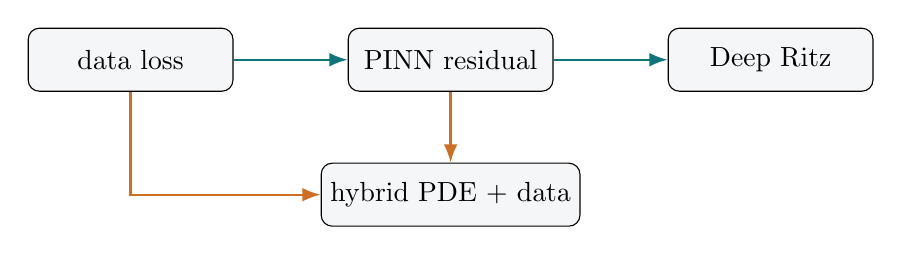
\begin{tikzpicture}[node distance=1.45cm,>=Latex]
\node[draw,rounded corners,fill=courseGrey,minimum width=2.6cm,minimum height=0.8cm] (data) {data loss};
\node[draw,rounded corners,fill=courseGrey,right=of data,minimum width=2.6cm,minimum height=0.8cm] (pinn) {PINN residual};
\node[draw,rounded corners,fill=courseGrey,right=of pinn,minimum width=2.6cm,minimum height=0.8cm] (ritz) {Deep Ritz};
\node[draw,rounded corners,fill=courseGrey,below=0.9cm of pinn,minimum width=3.1cm,minimum height=0.8cm] (hybrid) {hybrid PDE + data};
\draw[->,thick,courseTeal] (data) -- (pinn);
\draw[->,thick,courseTeal] (pinn) -- (ritz);
\draw[->,thick,courseOrange] (pinn) -- (hybrid);
\draw[->,thick,courseOrange] (data) |- (hybrid);
\end{tikzpicture}
\end{center}
\[
\inf_{\theta\in\Theta} \Loss(\theta)
\quad\leadsto\quad
\text{function } u_\theta: \Omega\to\R^{d_u}.
\]
\end{frame}

\renewcommand{\slideid}{L3-S003}
\begin{frame}[c]{The starting point: data-driven learning}
\small
\guidingquestion{What does a neural network learn before we use any PDE structure?}
\[
\D_d=\{(x_i^d,y_i)\}_{i=1}^{N_d},
\qquad x_i^d\in\R^d,\qquad y_i\in\R^{d_u} .
\]
\[
\widehat\Loss_d(\theta)=\frac1{N_d}\sum_{i=1}^{N_d}
\ell\bigl(u_\theta(x_i^d),y_i\bigr),
\qquad \text{train }\theta\in\Theta\text{ to reduce }\widehat\Loss_d.
\]
\begin{block}{Interpretation}
\begin{slideitems}
\item We start by fitting a nonlinear trial function to observations.
\end{slideitems}
\end{block}
\labnote{$d$ is the input dimension and $d_u$ the output dimension; most examples have $d_u=1$.}
\end{frame}

\renewcommand{\slideid}{L3-S005}
\begin{frame}[c]{Supervised PDE data: solution samples}
\small
\[
u_{tt}=u_{xx},\qquad u(t,x)=\sin(\pi x)\cos(\pi t),
\qquad x\in[0,1].
\]
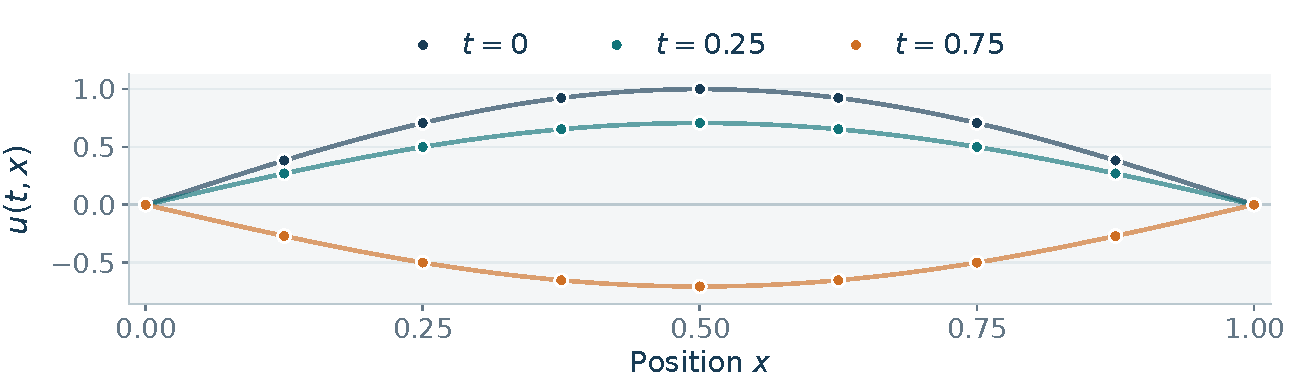
\includegraphics[width=\textwidth]{experiments/figures/wave_data.pdf}
\[
\D_d=\{(t_i^d,x_i^d,y_i)\}_{i=1}^{N_d},\qquad
\widehat\Loss_d(\theta)=\frac1{N_d}\sum_{i=1}^{N_d}
|u_\theta(t_i^d,x_i^d)-y_i|^2.
\]
\labnote{Synthetic noiseless samples $y_i=u(t_i^d,x_i^d)$, with fixed endpoints
$u(t,0)=u(t,1)=0$. Training uses only the samples: the PDE is absent from this loss.}
\end{frame}

\subsection{PDE-informed learning}
\renewcommand{\slideid}{L3-S008}
\begin{frame}[c]{Use the PDE to train the network}
\small
\guidingquestion{What changes when solution labels are unavailable but the governing equation is known?}
\[
\boxed{
\Lop u=f \quad\text{in }\Omega,
\qquad
\Bop u=g \quad\text{on }\partial\Omega
}
\]
\[
\begin{gathered}
\text{Solution labels }y_i\text{ are unavailable, but}\\
\Lop u_\theta(x_i^r)-f(x_i^r)\text{ can be evaluated.}
\end{gathered}
\]
\[
\theta \longmapsto u_\theta
\quad \text{parametrises a nonlinear ansatz class.}
\]
\begin{center}
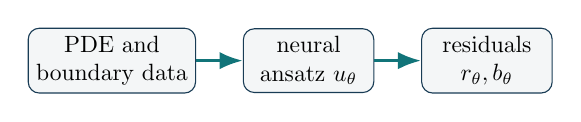
\begin{tikzpicture}[node distance=0.7cm,>=Latex,transform shape,scale=0.85]
\node[courseNode,minimum width=1.95cm] (equation) {PDE and\\boundary data};
\node[courseNode,minimum width=1.95cm,right=of equation] (network) {neural\\ansatz $u_\theta$};
\node[courseNode,minimum width=1.95cm,right=of network] (residual) {residuals\\$r_\theta,b_\theta$};
\draw[courseArrow] (equation) -- (network);
\draw[courseArrow] (network) -- (residual);
\end{tikzpicture}
\end{center}
\end{frame}

\section{Strong-form PINNs}
\subsection{Formulation and collocation}
\renewcommand{\slideid}{L3-S010}
\begin{frame}[c]{A running elliptic model problem}
\small
\guidingquestion{Which strong and weak notions of solution will we compare?}
\[
\begin{cases}
-\nabla\cdot(A(x)\nabla u)=f & \text{in }\Omega,\\
u=g_D & \text{on }\Gamma_D,\\
A\nabla u\cdot n=g_N & \text{on }\Gamma_N.
\end{cases}
\]
\[
A(x)\xi\cdot\xi\ge a_0|\xi|^2,
\qquad
\Omega\subset\R^d \text{ bounded Lipschitz}.
\]
\begin{block}{Two solution concepts}
\begin{slideitems}
\item Strong: pointwise derivatives.
\item Weak: variational derivatives.
\end{slideitems}
\end{block}
\end{frame}

\renewcommand{\slideid}{L3-S011}
\begin{frame}[c]{Classical discretisation versus neural ansatz}
\small
\[
V_h=\spanop\{\phi_1,\ldots,\phi_M\},
\qquad u_h=\sum_{j=1}^M c_j\phi_j.
\]
\[
\U_\Theta=\{u_\theta:\theta\in\Theta\},\qquad\Theta\subset\R^P.
\]
\[
u_\theta(x)=W_L\sigma(\cdots \sigma(W_1x+b_1)).
\]
\begin{center}
\begin{tabular}{lll}
\toprule
method & unknowns & geometry \\
\midrule
FEM/FDM & linear coefficients & mesh/stencil \\
NN PDE solver & nonlinear weights & sampled points \\
\bottomrule
\end{tabular}
\end{center}
\end{frame}

\renewcommand{\slideid}{L3-S012}
\begin{frame}[c]{Strong residual minimisation}
\small
\guidingquestion{How can the PDE itself become a loss function?}
\[
r_\theta(x)=\Lop[u_\theta](x)-f(x).
\]
\[
\Loss_r(\theta)=\norm{r_\theta}_{L^2(\Omega)}^2
=\int_\Omega |\Lop[u_\theta](x)-f(x)|^2\dd x.
\]
\[
\inf_{\theta\in\Theta}\Loss_r(\theta)\qquad\text{(attainment is a separate question).}
\]
\end{frame}

\renewcommand{\slideid}{L3-S013}
\begin{frame}[c]{From collocation points to the PINN objective}
\small
Choose interior points $X_r=\{x_i^r\}_{i=1}^{N_r}$ and boundary points
$X_b=\{x_i^b\}_{i=1}^{N_b}$, with positive quadrature weights.
\[
\begin{aligned}
\widehat\Loss_r(\theta)&=\sum_{i=1}^{N_r}w_i^r|r_\theta(x_i^r)|^2,\\[0.4em]
\widehat\Loss_b(\theta)&=\sum_{i=1}^{N_b}w_i^b|b_\theta(x_i^b)|^2,
\qquad b_\theta=\Bop u_\theta-g.
\end{aligned}
\]
\begin{block}{Balance the interior and boundary equations}
\[
\widehat\Loss_{\rm PINN}(\theta)
=\lambda_r\widehat\Loss_r(\theta)+\lambda_b\widehat\Loss_b(\theta).
\]
The positive weights $\lambda_r,\lambda_b$ set the relative scale and priority
of the two terms. Training returns parameters $\widehat\theta$.
\end{block}
\labnote{The continuous boundary loss is $\Loss_b=\norm{b_\theta}_{L^2(\partial\Omega)}^2$.
Uniform Monte Carlo uses $w_i^r=|\Omega|/N_r$ and $w_i^b=|\partial\Omega|/N_b$.}
\end{frame}

% Proofs and references: experiments/wellposedness_notes.md.
% These tanh constructions are independent of the Gaussian example in
% Zuazua, arXiv:2606.04018v2.

\renewcommand{\slideid}{L3-Q01}
\begin{frame}[c]{Question 1: is the neural minimum attained?}
\small
\guidingquestion{Even for a well-posed PDE, must a best neural-network solution exist?}
Consider the uniquely solvable problem
\[
 -u''=0\quad\text{in }(0,1),\qquad u(0)=0,\quad u(1)=1;
 \qquad u(x)=x.
\]
Fix any finite width $m\ge1$ and use a shallow tanh network:
\[
 u_\theta(x)=c+\sum_{j=1}^{m}a_j\tanh(b_jx+d_j).
\]
\[
 \Loss(v)=\int_0^1|v''(x)|^2\dd x
       +|v(0)|^2+|v(1)-1|^2.
\]
\begin{block}{Loss can approach zero without attaining it}
We will construct networks with loss tending to zero, while no finite
parameter vector attains zero loss.
\end{block}
\end{frame}

\renewcommand{\slideid}{L3-Q02}
\begin{frame}[c]{A tanh sequence approaches the infimum}
\small
One hidden neuron already gives the sequence
\[
 \boxed{v_n(x)=\frac{\tanh(x/n)}{\tanh(1/n)}},\qquad n=1,2,\ldots
\]
\[
 v_n(0)=0,\qquad v_n(1)=1,\qquad
 v_n\longrightarrow x\quad\text{in }C^2[0,1].
\]
Indeed, Taylor expansion yields
\[
 v_n(x)=x+\frac{x-x^3}{3n^2}+O(n^{-4}),\qquad
 v_n''(x)=-\frac{2x}{n^2}+O(n^{-4}).
\]
\[
 \Loss(v_n)=\frac{4}{3n^4}+O(n^{-6})\longrightarrow0.
\]
\begin{block}{The output weight diverges while the functions converge}
The output weight $a_1^{(n)}=1/\tanh(1/n)\sim n$ diverges.
The corresponding functions converge to the exact PDE solution.
\end{block}
\end{frame}

\renewcommand{\slideid}{L3-Q03}
\begin{frame}[c]{Why no finite tanh network attains this minimum}
\small
\begin{slideitems}
\item If $\Loss(u_\theta)=0$, then $u_\theta''=0$ and the endpoint data
force $u_\theta(x)=x$ throughout $(0,1)$.
\item A finite sum of tanh units is real analytic on $\R$.
Equality on an interval would therefore imply $u_\theta(x)=x$ on all of $\R$.
\item Every such finite tanh sum is bounded on $\R$; the function $x$ is
unbounded. This is a contradiction.
\end{slideitems}
\[
 \boxed{\inf_{\theta\in\Theta}\Loss(u_\theta)=0,
 \qquad \argmin_{\theta\in\Theta}\Loss(u_\theta)=\varnothing.}
\]
\begin{block}{Existence and approximation are different questions}
The PDE has a unique solution. The neural infimum is approached arbitrarily
well, but its limit lies outside this fixed finite tanh class.
\end{block}
\labnote{The conclusion depends on the stated architecture: adding a linear
skip connection makes $v(x)=x$ representable and removes this example.}
\end{frame}

\renewcommand{\slideid}{L3-Q04}
\begin{frame}[c]{Question 2: do small continuous residuals force convergence?}
\small
\guidingquestion{If $\Loss(u_{\theta_n})\to0$ for the exact integral loss, must
$u_{\theta_n}$ converge to the PDE solution in $L^2$?}
Consider the semilinear Neumann problem
\[
 -u''+\frac{u}{1+u^2}=0\quad\text{in }(0,1),
 \qquad u'(0)=u'(1)=0.
\]
Multiplying by $u$ and integrating gives
\[
 \int_0^1\left(|u'|^2+\frac{u^2}{1+u^2}\right)\dd x=0,
 \qquad\text{so the unique solution is }u=0.
\]
\begin{block}{The continuous residual loss}
\[
 \Loss(v)=\int_0^1\left|-v''+\frac{v}{1+v^2}\right|^2\dd x
             +|v'(0)|^2+|v'(1)|^2.
\]
\end{block}
\labnote{All integrals are exact. This example tests global residual-to-state stability,
without introducing sampling or quadrature.}
\end{frame}

\renewcommand{\slideid}{L3-Q05}
\begin{frame}[c]{Counterexample: vanishing continuous loss, diverging state}
\small
One tanh neuron represents a constant sequence:
\[
 v_n(x)=\frac{n}{\tanh(1)}\tanh(0x+1)=n,
 \qquad v_n'(0)=v_n'(1)=0.
\]
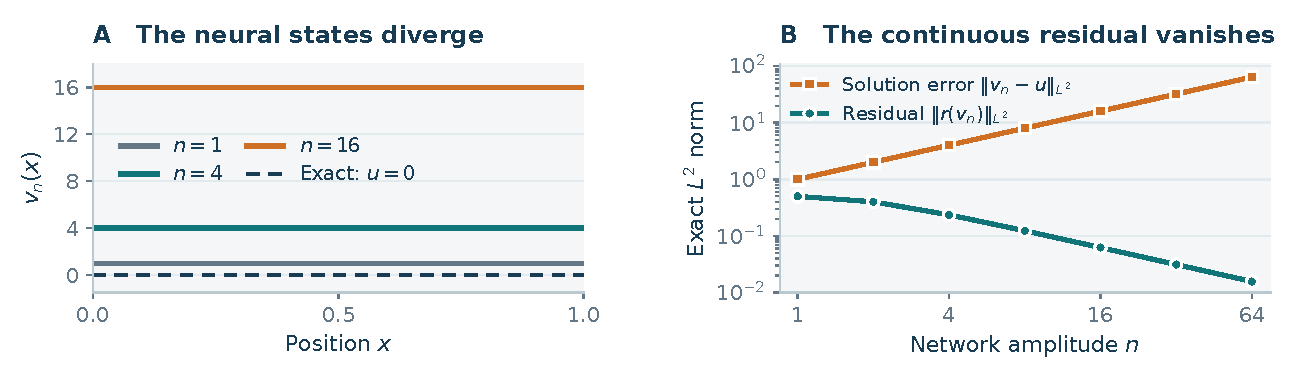
\includegraphics[width=\textwidth]{experiments/figures/continuous_residual.pdf}
\[
 \boxed{\Loss(v_n)=\frac{n^2}{(1+n^2)^2}\to0,
 \qquad \norm{v_n-u}_{L^2(0,1)}=n\to\infty.}
\]
\labnote{Uniqueness alone gives no global residual-to-error bound:
$s/(1+s^2)\to0$ as $s\to\infty$.}
\end{frame}
\renewcommand{\slideid}{L3}


\renewcommand{\slideid}{L3-S016}
\begin{frame}[c]{Example: Poisson PINN}
\small
\[
\begin{cases}
-\Delta u=f & \text{in }\Omega,\\
u=g & \text{on }\partial\Omega.
\end{cases}
\]
\[
r_\theta(x)=-\sum_{j=1}^d \partial_{x_jx_j}u_\theta(x)-f(x).
\]
\[
\begin{aligned}
\widehat\Loss_{\rm PINN}(\theta)
={}&\lambda_r\frac{|\Omega|}{N_r}\sum_{i=1}^{N_r}|r_\theta(x_i^r)|^2\\
&+\lambda_b\frac{|\partial\Omega|}{N_b}\sum_{i=1}^{N_b}|u_\theta(x_i^b)-g(x_i^b)|^2.
\end{aligned}
\]
\end{frame}

\renewcommand{\slideid}{L3-S017}
\begin{frame}[c]{Example: heat equation PINN}
\small
\[
\begin{cases}
\partial_t u-\kappa\Delta u=f & \text{in }Q=(0,T)\times\Omega,\\
u(0,x)=u_0(x) & x\in\Omega,\\
\Bop u=g & \text{on }\Sigma=(0,T)\times\partial\Omega.
\end{cases}
\]
\[
r_\theta(t,x)=\partial_t u_\theta(t,x)-\kappa\Delta_xu_\theta(t,x)-f(t,x).
\]
\[
\begin{aligned}
\Loss(\theta)={}&\lambda_r\norm{r_\theta}_{L^2(Q)}^2
+\lambda_0\norm{u_\theta(0,\cdot)-u_0}_{L^2(\Omega)}^2\\
&+\lambda_b\norm{\Bop u_\theta-g}_{L^2(\Sigma)}^2.
\end{aligned}
\]
\labnote{$\Sigma=(0,T)\times\partial\Omega$ is the lateral boundary; $u_0$ is the initial datum.}
\end{frame}

\subsection{Quadrature, stability, and error}
\renewcommand{\slideid}{L3-S019}
\begin{frame}[c]{Approximating the residual integral}
\small
\[
\Loss_r(\theta)=\int_\Omega |r_\theta(x)|^2\dd x.
\]
\[
\widehat\Loss_r(\theta)=\sum_{i=1}^{N_r}w_i^r |r_\theta(x_i^r)|^2.
\]
\[
\underbrace{\Loss_r(\widehat\theta)}_{\text{continuum residual}}
\quad\text{need not equal}\quad
\underbrace{\widehat\Loss_r(\widehat\theta)}_{\text{training residual}}
\]
\labnote{Relating the two requires control of the quadrature error.}
\end{frame}

\renewcommand{\slideid}{L3-S020}
\begin{frame}[c]{Two ways to approximate the residual integral}
\small
For $\varphi_\theta=|r_\theta|^2$, write
$I(\varphi)=\int_\Omega\varphi\dd x$.
\begin{block}{Deterministic quadrature: regularity controls the error}
\[
Q_N(\varphi)=\sum_{i=1}^Nw_i\varphi(x_i),\qquad
|I(\varphi)-Q_N(\varphi)|\le Ch^q\norm{\varphi}_{W^{q,1}(\Omega)}.
\]
Resolving the network values alone is insufficient: derivatives of the
squared residual enter the quadrature estimate.
\end{block}
\begin{block}{Monte Carlo: variance controls the error}
\[
x_i\overset{\rm iid}{\sim}\operatorname{Unif}(\Omega),\qquad
\widehat I_N(\varphi)=\frac{|\Omega|}{N}\sum_{i=1}^N\varphi(x_i).
\]
\[
\E[\widehat I_N]=I(\varphi),\qquad
\Var[\widehat I_N]=\frac{|\Omega|^2}{N}\Var[\varphi(X)].
\]
The root-mean-square rate is $N^{-1/2}$; its constant depends on the variance.
\end{block}
\end{frame}

\renewcommand{\slideid}{L3-S023}
\begin{frame}[c]{Residual norm versus solution error}
\small
\guidingquestion{When does a small residual actually imply a small solution error?}
\[
e_\theta=u_\theta-u.
\]
\[
\Lop e_\theta=r_\theta,
\qquad \Bop e_\theta=b_\theta.
\]
\labnote{These residual identities assume linear operators $\Lop$ and $\Bop$.}
\[
\norm{e_\theta}_{X}
\le C_{\rm stab}
\bigl(\norm{r_\theta}_{Y}+\norm{b_\theta}_{Z}\bigr)
\]
\begin{block}{Key point}
\begin{slideitems}
\item A stability estimate tells us when the residual controls solution error.
\end{slideitems}
\end{block}
\end{frame}

\renewcommand{\slideid}{L3-S024}
\begin{frame}[c]{When a strong residual requires too much regularity}
\small
\[
\Lop:H^{s}(\Omega)\to L^2(\Omega)
\quad\text{requires } u\in H^{s}(\Omega).
\]
\[
-\Delta u=f \text{ in } L^2
\quad\Rightarrow\quad u\in H^2(\Omega)
\text{ only under regularity assumptions.}
\]
\[
\begin{gathered}
f\in L^2(\Omega)\text{ still gives }\Delta u=-f\in L^2(\Omega),\\
\text{but on a nonconvex domain, }u\in H^2(\Omega)\text{ may fail.}
\end{gathered}
\]
\end{frame}

\subsection{Training and approximation limits}
\renewcommand{\slideid}{L3-S026}
\begin{frame}[c]{Why the loss can be nonconvex}
\small
Even for a linear PDE, the network depends nonlinearly on its parameters.
The loss depends on the parameters through:
\[
\theta\mapsto u_\theta\mapsto\Lop u_\theta
\mapsto\norm{\Lop u_\theta-f}_{L^2(\Omega)}^2.
\]
\medskip
The loss need not satisfy the convexity inequality:
\[
\Loss(\alpha\theta_1+(1-\alpha)\theta_2)
\not\le\alpha\Loss(\theta_1)+(1-\alpha)\Loss(\theta_2).
\]
\labnote{The inequality can fail for some $\theta_1,\theta_2$ and $0<\alpha<1$;
interpolating weights does not interpolate network outputs.}
\medskip
\begin{block}{What this means for training}
The final loss depends on initialization and the optimizer.
Check the PDE error even when the parameter gradient is small.
\end{block}
\[
\theta_K=\operatorname{Optimizer}_K(\theta_0,\widehat\Loss,\eta,\text{batching}).
\]
\labnote{$K$ is the number of updates and $\eta$ the learning rate;
training uses the sampled objective $\widehat\Loss$.}
\end{frame}

\renewcommand{\slideid}{L3-S028}
\begin{frame}[c]{Optimization error}
\small
\[
\begin{aligned}
\Loss(\theta_K)-\inf_{\theta\in\Theta}\Loss(\theta)
={}&\underbrace{\Loss(\theta_K)-\widehat\Loss(\theta_K)}_{\text{quadrature/generalization}}\\[1.1em]
&+\underbrace{\widehat\Loss(\theta_K)
-\inf_{\theta\in\Theta}\widehat\Loss(\theta)}_{\text{optimization}}\\[1.1em]
&+\underbrace{\inf_{\theta\in\Theta}\widehat\Loss(\theta)
-\inf_{\theta\in\Theta}\Loss(\theta)}_{\text{quadrature bias}}.
\end{aligned}
\]
\end{frame}

\renewcommand{\slideid}{L3-S029}
\begin{frame}[c]{Training loss and the full PDE error budget}
\small
\[
\widehat\Loss(\theta_K)\downarrow
\quad\not\Longrightarrow\quad
\norm{u_{\theta_K}-u}_{X}\downarrow.
\]
\begin{block}{Sources of PDE error}
\[
\begin{aligned}
\text{PDE error}\lesssim{}&\text{approximation}+\text{quadrature}\\
&+\text{optimization}+\text{penalty}+\text{modeling}.
\end{aligned}
\]
\end{block}
\begin{slideitems}
\item A stability estimate must turn the chosen residual into a state-error bound.
\item Quadrature and boundary control must remain reliable for the trained network.
\item Successful optimization reduces only one part of the error budget;
architecture, sampling, and model accuracy affect the other parts.
\end{slideitems}
\end{frame}

% Computed figures and metrics are generated by experiments/make_figures.py.
\renewcommand{\slideid}{L3-PY01}
\begin{frame}[c]{Python lab 1: solve Poisson without solution labels}
\small
\[
 -u''=\pi^2\sin(\pi x),\quad x\in(0,1),\qquad u(0)=u(1)=0.
\]
\lstinputlisting[style=pythonlab]{experiments/snippets/forward_setup.py}
\begin{block}{Network and training setup}
Use $u_\theta=x(1-x)N_\theta$, with raw network $N_\theta$;
seed 7, float64 on CPU.
Use the exact solution $u=\sin(\pi x)$ to evaluate the error after training.
\end{block}
\end{frame}

\renewcommand{\slideid}{L3-PY02}
\begin{frame}[c]{Python lab 1: differentiate, form the loss, train}
\small
\lstinputlisting[style=pythonlab]{experiments/snippets/forward_loss.py}
Differentiate network values (\texttt{u}) in $x$ for the residual, and in $\theta$ to train.\par\medskip
\labnote{\ForwardProtocol. Residual divided by $\pi^2$; boundaries enforced by $x(1-x)$.}
\end{frame}

\renewcommand{\slideid}{L3-PY03}
\begin{frame}[c]{Python output: inspect the solution and its error}
\small
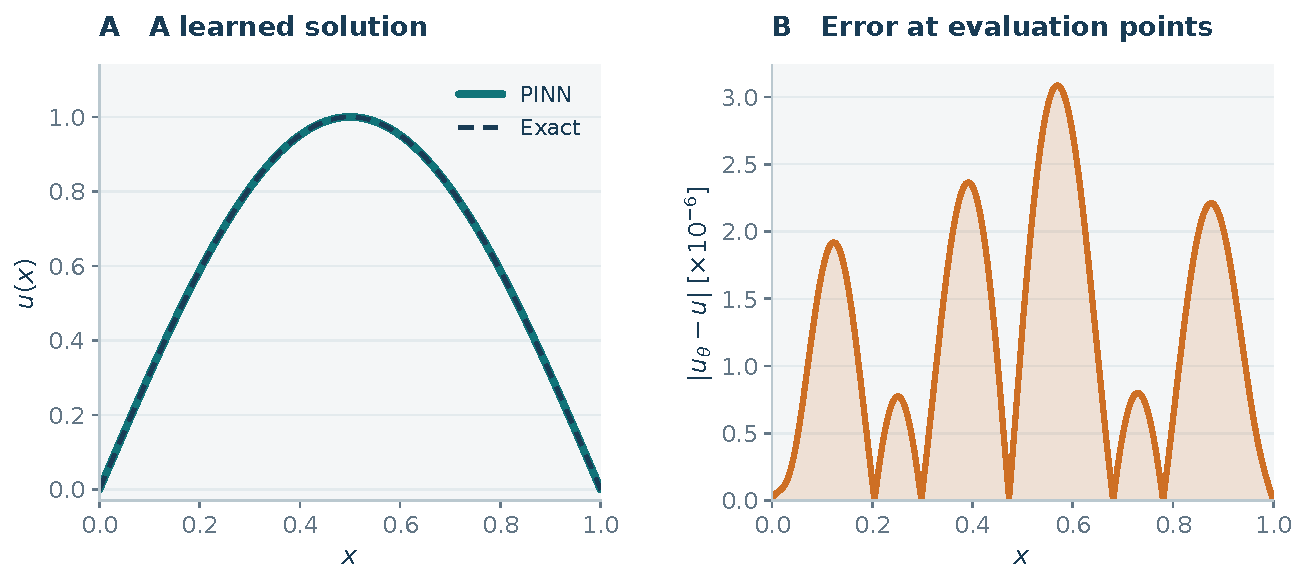
\includegraphics[width=\textwidth]{experiments/figures/poisson_1d.pdf}
\begin{block}{Measured on 1,001 evaluation points}
Relative $L^2$ error: \textbf{\ForwardLtwo}; maximum absolute error:
\textbf{\ForwardMaxError}. The endpoints are exactly zero by construction.
\end{block}
\labnote{The error panel resolves differences hidden by overlapping solution curves.
All reported errors are numerical grid estimates.}
\end{frame}

\renewcommand{\slideid}{L3-PY04}
\begin{frame}[c]{Python lab 2: the same idea in two dimensions}
\small
\[
 -\Delta u=2\pi^2\sin(\pi x)\sin(\pi y),\qquad
 u|_{\partial(0,1)^2}=0.
\]
\lstinputlisting[style=pythonlab]{experiments/snippets/poisson_2d_loss.py}
\end{frame}

\renewcommand{\slideid}{L3-PY05}
\begin{frame}[c]{Python output: a field, a reference, an error map}
\small
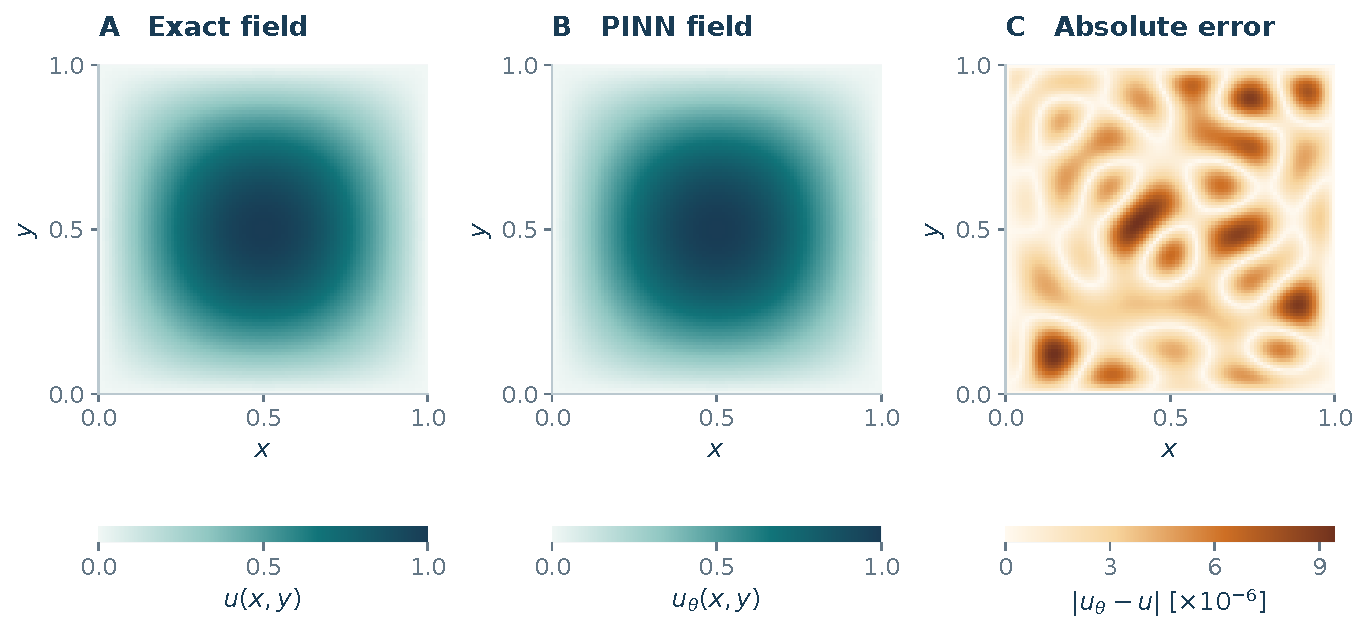
\includegraphics[width=\textwidth]{experiments/figures/poisson_2d.pdf}
\begin{block}{Validate on a separate $101\times101$ mesh}
Relative $L^2$ error: \textbf{\TwoDLtwo}; maximum absolute error:
\textbf{\TwoDMaxError}.
\end{block}
\labnote{Exact and learned fields share one color scale. The error uses its own
scale to reveal where the approximation is least accurate.}
\end{frame}
\renewcommand{\slideid}{L3}


\section{Network design and boundary constraints}
\subsection{Regularity and architecture}
\renewcommand{\slideid}{L3-S032}
\begin{frame}[c]{Activation functions: derivative order matters}
\small
\guidingquestion{How smooth must the network be for the chosen differential operator?}
\[
\Lop \text{ contains derivatives up to order }s.
\]
\[
\begin{gathered}
\text{A pointwise residual needs derivatives through order }s\\
\text{at the collocation points.}
\end{gathered}
\]
\[
\sigma\in C^s\quad\Rightarrow\quad u_\theta\in C^s(\Omega)
\quad\text{is sufficient for these derivatives to exist.}
\]
\end{frame}

\renewcommand{\slideid}{L3-S033}
\begin{frame}[c]{ReLU: classical derivatives and distributional derivatives}
\small
\[
\sigma(z)=\max\{0,z\},\qquad
\sigma'(z)=\mathbf1_{z>0},\qquad \sigma''(z)=0\quad\text{a.e.}
\]
A ReLU network is piecewise affine. Inside each linear region,
$D^2u_\theta=0$, so its classical Laplacian cannot match a smooth nonzero forcing.
\begin{block}{The missing second derivative lives at the kinks}
\[
D^2\operatorname{ReLU}=\delta_0\qquad\text{in distributions.}
\]
Automatic differentiation usually returns zero away from the kinks;
it does not return this singular measure.
\end{block}
\medskip
Thus a strong second-order residual can miss the network's singular
second derivatives, even when its values look accurate.
\end{frame}

\renewcommand{\slideid}{L3-S035}
\begin{frame}[c]{When ReLU can still be sensible}
\small
\[
\text{First-order PDE: } \Lop u=b\cdot\nabla u+cu.
\]
\[
\text{Weak formulations: derivatives are shifted to tests.}
\]
\[
\text{Deep Ritz for Poisson: } \Energy(v)=\frac12\int_\Omega|\nabla v|^2\dd x-\int_\Omega fv\dd x.
\]
\[
\nabla u_\theta \in L^\infty \text{ piecewise constant is admissible in }H^1.
\]
\end{frame}

\renewcommand{\slideid}{L3-S036}
\begin{frame}[c]{Choose the activation for the formulation}
\small
\[
\begin{array}{lll}
\tanh z &:& C^\infty,\ \text{saturating},\\[0.25em]
\operatorname{softplus}_\beta(z)=\beta^{-1}\log(1+e^{\beta z}) &:& C^\infty,\\[0.25em]
\sin(\omega z) &:& C^\infty,\ \text{oscillatory},\\[0.25em]
z\sigma_{\rm sigmoid}(z) &:& \text{SiLU/Swish, smooth}.
\end{array}
\]
\begin{block}{Match the derivatives used by the loss}
For a strong residual of order $s$, choose $\sigma\in C^s$ with numerically
stable derivatives through order $s$.
\medskip

Poisson energy needs only first derivatives:
$\sigma\in W^{1,\infty}_{\rm loc}(\R)$ suffices for $u_\theta\in H^1(\Omega)$
on a bounded domain.
\end{block}
\labnote{Smoothness makes the derivatives available; it does not guarantee good conditioning.}
\end{frame}

\subsection{Boundary conditions}
\renewcommand{\slideid}{L3-S043}
\begin{frame}[c]{Boundary constraints and the Dirichlet penalty}
\small
The constrained problem is
\[
\inf_{v\in X}\Loss_r(v)\quad\text{subject to}\quad\Bop v=g.
\]
A penalty replaces exact feasibility by a weighted boundary mismatch.
For $u=g_D$ on $\Gamma_D\subset\partial\Omega$,
\[
\Loss_D(\theta)=\int_{\Gamma_D}|u_\theta-g_D|^2\dd s,
\]
\[
\widehat\Loss_D(\theta)=\sum_{i=1}^{N_D}w_i^D
|u_\theta(x_i^D)-g_D(x_i^D)|^2\approx\Loss_D(\theta).
\]
\begin{block}{Soft enforcement}
\[
\Loss(\theta)=\Loss_r(\theta)+\lambda_D\Loss_D(\theta).
\]
Finite $\lambda_D$ trades interior fit against boundary accuracy.
The exact constraint is recovered only in an ideal penalty limit.
\end{block}
\labnote{The subscript $D$ identifies the Dirichlet boundary; $x_i^D\in\Gamma_D$.}
\end{frame}

\renewcommand{\slideid}{L3-S045}
\begin{frame}[c]{Neumann and Robin penalties}
\small
\[
A\nabla u\cdot n=g_N
\quad\Rightarrow\quad
\Loss_N(\theta)=\int_{\Gamma_N}|A\nabla u_\theta\cdot n-g_N|^2\dd s.
\]
\[
\alpha u+A\nabla u\cdot n=g_R
\quad\Rightarrow\quad
\Loss_R(\theta)=\int_{\Gamma_R}|\alpha u_\theta+A\nabla u_\theta\cdot n-g_R|^2\dd s.
\]
\end{frame}

\renewcommand{\slideid}{L3-S046}
\begin{frame}[c]{Initial conditions are boundary conditions in space-time}
\small
\[
Q=(0,T)\times\Omega,
\qquad \Sigma_0=\{0\}\times\Omega,\quad \Sigma=(0,T)\times\partial\Omega.
\]
\[
\Loss_0(\theta)=\int_\Omega |u_\theta(0,x)-u_0(x)|^2\dd x.
\]
\[
\Loss(\theta)=\lambda_r\Loss_r(\theta)+\lambda_0\Loss_0(\theta)+\lambda_b\Loss_b(\theta).
\]
\end{frame}

\renewcommand{\slideid}{L3-S047}
\begin{frame}[c]{Penalty parameter asymptotics}
\small
\[
\theta_{\lambda_b}\in\argmin_{\theta\in\Theta}
\bigl(\Loss_r(\theta)+\lambda_b\Loss_b(\theta)\bigr).
\]
\[
\lambda_b\uparrow\infty:
\qquad
\Loss_b(\theta_{\lambda_b})\downarrow
\quad\text{but conditioning deteriorates.}
\]
\[
\nabla_\theta\Loss=\nabla_\theta\Loss_r+\lambda_b\nabla_\theta\Loss_b.
\]
\labnote{This ideal comparison assumes exact minimisers exist for each $\lambda_b$.}
\end{frame}

\renewcommand{\slideid}{L3-S049}
\begin{frame}[c]{Encode Dirichlet data directly in the network}
\small
Let $N_\theta$ be an unconstrained network. Choose a lifting $G$ and a
boundary-vanishing factor $\rho$ such that
\[
G|_{\partial\Omega}=g,\qquad \rho|_{\partial\Omega}=0,
\qquad \rho>0\ \text{in }\Omega.
\]
\[
\boxed{u_\theta(x)=G(x)+\rho(x)N_\theta(x)}
\quad\Longrightarrow\quad u_\theta|_{\partial\Omega}=g.
\]
\begin{block}{Homogeneous data are the special case $G=0$}
Then $u_\theta=\rho N_\theta$ satisfies zero Dirichlet data for every $\theta$.
The training objective only needs the interior residual:
\[
\Loss_r(\theta)=\int_\Omega
|\Lop[G+\rho N_\theta]-f|^2\dd x.
\]
\end{block}
\labnote{Boundary enforcement is exact when $G$ and $\rho$ satisfy their trace conditions exactly.}
\end{frame}

\renewcommand{\slideid}{L3-S052}
\begin{frame}[c]{Hard constraints on boxes and in time}
\small
\begin{block}{Zero Dirichlet data on the unit box}
\[
\Omega=(0,1)^d,\qquad \rho(x)=\prod_{j=1}^d x_j(1-x_j),
\]
\[
u_\theta(x)=\rho(x)N_\theta(x)\quad\Longrightarrow\quad
u_\theta|_{\partial\Omega}=0.
\]
\end{block}
\begin{block}{Initial data and compatible spatial boundary data}
For $u(0,x)=u_0(x)$, use $u_\theta(t,x)=u_0(x)+tN_\theta(t,x)$.
To encode both initial and boundary conditions, use
\[
u_\theta(t,x)=G(t,x)+t\rho(x)N_\theta(t,x).
\]
Choose $G(0,x)=u_0(x)$ and $G=g$ on the spatial boundary.
\end{block}
\labnote{The initial and boundary data must be compatible where their boundaries meet.}
\end{frame}

\renewcommand{\slideid}{L3-S055}
\begin{frame}[c]{Boundary penalties versus hard constraints}
\small
\begin{center}
\footnotesize
\begin{tabular}{lll}
\toprule
approach & advantage & risk \\
\midrule
penalty & easy, general & tuning, constraint drift \\
hard encoding & exact Dirichlet & geometry, regularity, expressivity \\
Nitsche/weak & variationally consistent & more derivation, parameters \\
\bottomrule
\end{tabular}
\end{center}
\[
\text{Choose based on geometry, regularity, and boundary accuracy.}
\]
\end{frame}

\renewcommand{\slideid}{L3-PY06}
\begin{frame}[c]{Python lab 3: sweep the boundary penalty}
\small
Keep the 1D Poisson problem; replace $x(1-x)N_\theta(x)$ by $N_\theta(x)$.
\lstinputlisting[style=pythonlab]{experiments/snippets/boundary_loss.py}
\begin{block}{Change one setting at a time}
$\lambda_b\in\{0.01,0.1,1,10,100,1000\}$; identical initial weights,
collocation points, learning rate, and \BoundarySteps\ Adam updates.
The hard-constraint run gets the same update budget.
\end{block}
\labnote{The residual is divided by $\pi^2$, so the weight sweep refers to that
specific scaling. No L-BFGS refinement is used in this comparison.}
\end{frame}

\renewcommand{\slideid}{L3-PY07}
\begin{frame}[c]{Python output: boundary accuracy is only one diagnostic}
\small
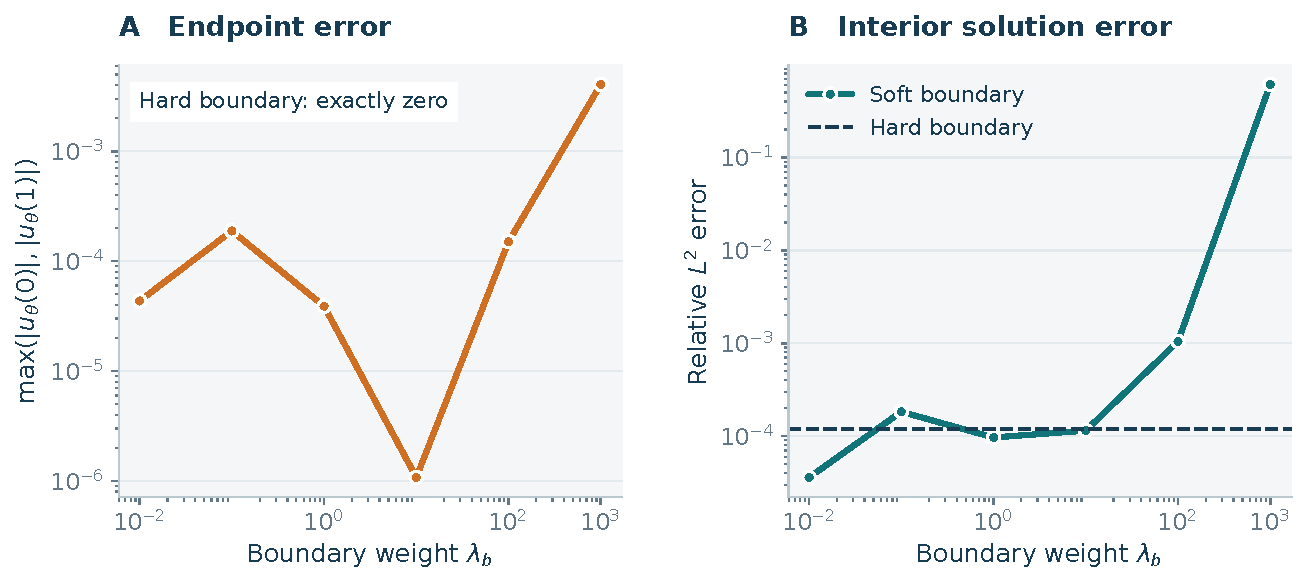
\includegraphics[width=\textwidth]{experiments/figures/boundary_sweep.pdf}
\begin{block}{Read both panels together}
Check the interior error as well as the boundary error.
The hard-constraint baseline has zero endpoint error exactly.
\end{block}
\labnote{These results use one seed and one training budget. Repeat the sweep
with other settings before choosing a penalty weight.}
\end{frame}
\renewcommand{\slideid}{L3}


\section{Variational and weak methods}
\subsection{Deep Ritz methods}
\renewcommand{\slideid}{L3-S058}
\begin{frame}[c]{From a weak formulation to an energy}
\small
For homogeneous Dirichlet data, take $V=H^1_{\Gamma_D}(\Omega)$ and seek
\[
u\in V:\qquad a(u,v)=F(v)\quad\forall v\in V,
\]
\[
\begin{aligned}
a(u,v)&=\int_\Omega A\nabla u\cdot\nabla v+cuv\dd x,\\
F(v)&=\int_\Omega fv\dd x+\int_{\Gamma_N}g_Nv\dd s.
\end{aligned}
\]
If $a$ is symmetric, continuous and coercive, define
\[
\Energy(v)=\tfrac12a(v,v)-F(v),
\qquad \delta\Energy(u)[v]=a(u,v)-F(v).
\]
\[
\boxed{u\in\argmin_{v\in V}\Energy(v)}
\quad\Longleftrightarrow\quad \text{the weak PDE.}
\]
\labnote{Nonzero Dirichlet data require a lifting and minimisation over the corresponding affine space.}
\end{frame}

\renewcommand{\slideid}{L3-S060}
\begin{frame}[c]{Poisson energy}
\small
\[
-\Delta u=f,
\qquad u|_{\partial\Omega}=0.
\]
\[
V=H_0^1(\Omega),
\qquad
\Energy(v)=\frac12\int_\Omega |\nabla v|^2\dd x
-\int_\Omega fv\dd x.
\]
\[
\delta \Energy(u)[v]=\int_\Omega\nabla u\cdot\nabla v\dd x-
\int_\Omega fv\dd x.
\]
\end{frame}

\renewcommand{\slideid}{L3-S061}
\begin{frame}[c]{Deep Ritz: train with first derivatives}
\small
Choose an admissible neural trial class and approximate the Poisson energy:
\[
\U_\Theta\subset V,
\qquad
\widehat\theta\in\Theta:\quad\text{trained to reduce }\widehat\Energy(u_\theta).
\]
\[
\widehat\Energy(u_\theta)=\frac12\sum_{i=1}^Nw_i|\nabla u_\theta(x_i)|^2
-\sum_{i=1}^Nw_i f(x_i)u_\theta(x_i).
\]
\begin{block}{What changes from a strong PINN?}
\begin{slideitems}
\item The Poisson residual requires $\Delta u_\theta$; the energy only requires $\nabla u_\theta$.
\item First derivatives lower the regularity required of the trial functions.
\item No labelled solution data are used: $f$, the domain and boundary conditions define the training objective.
\end{slideitems}
\end{block}
\end{frame}

\renewcommand{\slideid}{L3-S063}
\begin{frame}[c]{Energy excess controls solution error}
\small
For the exact weak solution $u$ and any admissible $v$, stationarity cancels the linear error term:
\[
\Energy(v)-\Energy(u)
=\tfrac12 a(v-u,v-u)
=\tfrac12\norm{v-u}_a^2.
\]
\[
\norm{e}_{a}^2:=a(e,e),\qquad
\alpha\norm{e}_V^2\le\norm{e}_a^2\le M\norm{e}_V^2.
\]
\[
\boxed{
\norm{v-u}_{V}
\le \alpha^{-1/2}\norm{v-u}_{a}
=\sqrt{\frac{2}{\alpha}\bigl(\Energy(v)-\Energy(u)\bigr)}
}
\]
\medskip
The energy gap is exactly a squared energy-norm error. Coercivity transfers this control to the desired Sobolev norm.
\end{frame}

\renewcommand{\slideid}{L3-S065}
\begin{frame}[c]{Coercivity from ellipticity}
\small
\[
A(x)\xi\cdot\xi\ge a_0|\xi|^2,
\qquad c(x)\ge0.
\]
\[
a(v,v)=\int_\Omega A\nabla v\cdot\nabla v+c v^2\dd x
\ge a_0\norm{\nabla v}_{L^2}^2.
\]
\[
V=H_0^1(\Omega):
\quad
\norm{v}_{L^2}\le C_P\norm{\nabla v}_{L^2}.
\]
Thus $a(v,v)\ge \frac{a_0}{1+C_P^2}\norm{v}_{H^1}^2$:
ellipticity controls gradients, and the Dirichlet condition controls constants.
\end{frame}

\renewcommand{\slideid}{L3-S066}
\begin{frame}[c]{Best approximation in energy norm}
\small
\[
u_\Theta^\star\in\argmin_{v\in\U_\Theta}\Energy(v).
\]
\[
\Energy(u_\Theta^\star)-\Energy(u)
=\frac12\norm{u_\Theta^\star-u}_{a}^2.
\]
\[
\text{Deep Ritz inherits the approximation properties of }\U_\Theta\text{ in }H^1.
\]
\labnote{Here $u_\Theta^\star$ denotes a best neural approximation, assuming the infimum is attained.}
\end{frame}

\renewcommand{\slideid}{L3-S070}
\begin{frame}[c]{Boundary penalty in Deep Ritz}
\small
\[
\Energy_{\lambda_b}(v)=\Energy(v)+\frac{\lambda_b}{2}
\int_{\partial\Omega}|v-g|^2\dd s.
\]
\[
\begin{aligned}
\delta \Energy_{\lambda_b}(v)[w]={}&a(v,w)-F(w)\\
&+\lambda_b\int_{\partial\Omega}(v-g)w\dd s.
\end{aligned}
\]
\[
\lambda_b<\infty
\quad\Rightarrow\quad
\text{Dirichlet data imposed weakly, not exactly.}
\]
\end{frame}

\renewcommand{\slideid}{L3-S072}
\begin{frame}[c]{Natural boundary conditions in energy form}
\small
\[
\begin{aligned}
\Energy(v)={}&\frac12\int_\Omega A\nabla v\cdot\nabla v\dd x\\
&-\int_\Omega fv\dd x-\int_{\Gamma_N}g_Nv\dd s.
\end{aligned}
\]
\[
\delta \Energy(u)[w]=0
\quad\Rightarrow\quad
A\nabla u\cdot n=g_N \text{ on }\Gamma_N.
\]
\[
\text{Neumann data are natural; Dirichlet data are essential.}
\]
\end{frame}

\renewcommand{\slideid}{L3-S074}
\begin{frame}[c]{Deep Ritz for nonlinear energies}
\small
\[
\Energy(v)=\int_\Omega W(\nabla v,v,x)\dd x-
\int_\Omega fv\dd x.
\]
\[
\delta \Energy(u)[w]=0
\quad\Rightarrow\quad
-\nabla\cdot W_p(\nabla u,u,x)+W_z(\nabla u,u,x)=f.
\]
\[
\text{Nonconvex }W\text{ can create multiple stationary points.}
\]
\labnote{$W_p$ and $W_z$ are derivatives with respect to the gradient and state arguments of $W(p,z,x)$.}
\end{frame}

\renewcommand{\slideid}{L3-S075}
\begin{frame}[c]{Two ways coercivity can weaken in practice}
\small
\textbf{Sampling.} A continuum energy can control the state error,
\[
\Energy(v)-\Energy(u)\ge c\norm{v-u}_{V}^2,
\]
while a sampled objective has no corresponding guarantee without further control:
\[
\widehat\Energy(v)-\widehat\Energy(u_{\widehat\theta})
\not\ge c\norm{v-u_{\widehat\theta}}_{V}^2\quad\text{in general.}
\]
\medskip
\textbf{Boundary penalty.} Gradients and traces control $H^1$:
\[
\Energy_{\lambda_b}(v)=\tfrac12\norm{\nabla v}_{L^2}^2-\int_\Omega fv\dd x
+\tfrac{\lambda_b}{2}\norm{v-g}_{L^2(\partial\Omega)}^2.
\]
A small $\lambda_b$ gives weak control of constants and boundary modes.
\par\smallskip
\labnote{In the sampled comparison, $u_{\widehat\theta}$ denotes a minimiser, if one exists.}
\end{frame}

\renewcommand{\slideid}{L3-PY08}
\begin{frame}[c]{Python lab 4: replace the strong residual by energy}
\small
For the same Poisson problem and hard Dirichlet ansatz,
\[
 \Energy(u_\theta)=\int_0^1\left[\tfrac12(u_\theta')^2
           -\pi^2\sin(\pi x)u_\theta\right]\dd x.
\]
\lstinputlisting[style=pythonlab]{experiments/snippets/ritz_loss.py}
\begin{block}{First derivatives suffice}
Use Gauss--Legendre nodes and weights on $[0,1]$.
The same network initialization isolates the change of objective.
\end{block}
\labnote{\RitzProtocol.}
\end{frame}

\renewcommand{\slideid}{L3-PY09}
\begin{frame}[c]{Python output: compare errors, not raw loss values}
\small
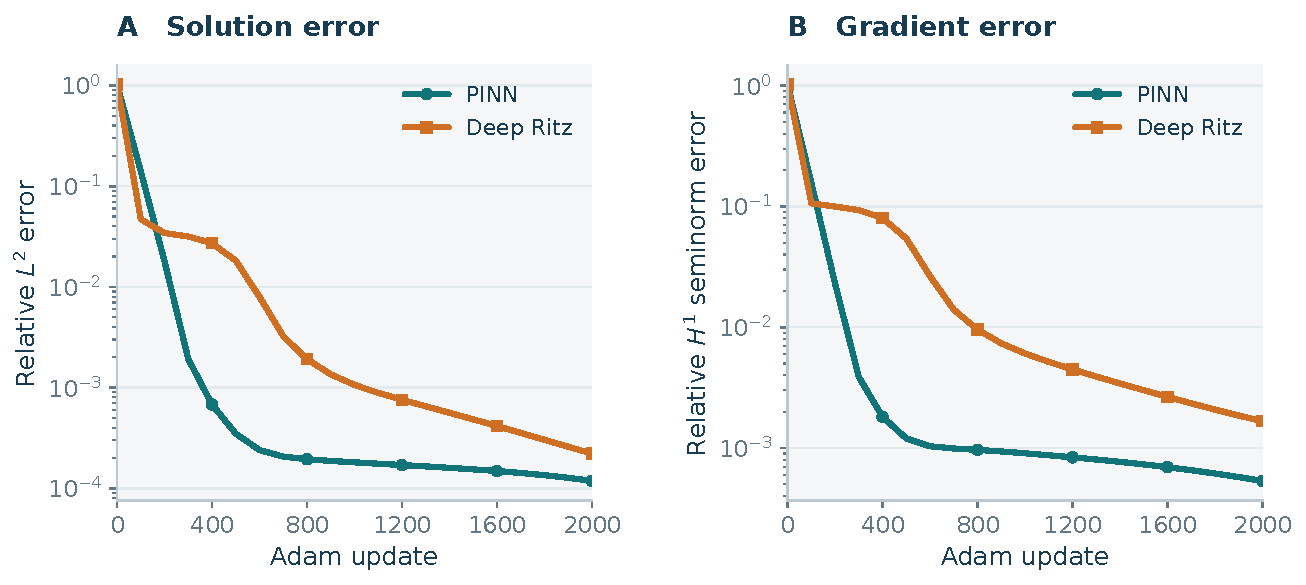
\includegraphics[width=\textwidth]{experiments/figures/ritz_comparison.pdf}
\begin{block}{Final evaluation after optimizer refinement}
\begin{tabular}{@{}lcc@{}}
 & relative $L^2$ error & relative $H^1$ seminorm error\\
PINN & \ForwardLtwo & \ForwardHone\\
Deep Ritz & \RitzLtwo & \RitzHone
\end{tabular}
\end{block}
\labnote{Curves show Adam only; the table includes subsequent L-BFGS refinement.
Equal updates do not imply equal runtime. One seed, one smooth problem.}
\end{frame}
\renewcommand{\slideid}{L3}


\subsection{Weak formulations}
\renewcommand{\slideid}{L3-S082}
\begin{frame}[c]{Weak residuals and finite test spaces}
\small
A weak formulation transfers derivatives to test functions and can accommodate
solutions without classical second derivatives:
\[
\WeakRes_\theta(v)=a(u_\theta,v)-F(v),\qquad v\in V.
\]
The exact solution satisfies $a(u,v)=F(v)$ for every $v\in V$. For pure diffusion
and $v_j\in H_0^1(\Omega)$, the neural residual moments are
\[
\WeakRes_\theta(v_j)=\int_\Omega A\nabla u_\theta\cdot\nabla v_j\dd x
-\int_\Omega fv_j\dd x.
\]
Choose a finite collection of tests and minimise
\[
\Loss_{\rm weak}(\theta)=\frac1M\sum_{j=1}^M|\WeakRes_\theta(v_j)|^2.
\]
This tests selected directions, rather than every direction in $V$.
\par\medskip
\labnote{The moments above are exact integrals. Numerical quadrature produces $\widehat\Loss_{\rm weak}$.}
\end{frame}

\renewcommand{\slideid}{L3-S085}
\begin{frame}[c]{Variational PINNs: neural trials and polynomial tests}
\small
Variational PINNs use spatially extended, admissible tests, often
polynomials. The trial family and test space play different roles:
\[
\U_\Theta=\{u_\theta:\theta\in\Theta\},\qquad
V_M=\spanop\{v_1,\ldots,v_M\}\subset V.
\]
\[
\Loss_{\rm VPINN}(\theta)=\frac1M\sum_{j=1}^M
|\WeakRes_\theta(v_j)|^2.
\]
This has a Petrov--Galerkin structure: a nonlinear neural trial family and a
fixed test space. The choice of tests determines which residual features are detected.
\end{frame}

\renewcommand{\slideid}{L3-S087}
\begin{frame}[c]{Local variational residuals and hp-refinement}
\small
Partition $\Omega$ into cells $K\in\mathcal T_h$, while keeping a global neural
trial function. For local tests vanishing on $\partial K$,
\[
\WeakRes_{\theta,K}(v_{K,j})=\int_K A\nabla u_\theta\cdot\nabla v_{K,j}\dd x
-\int_K fv_{K,j}\dd x,
\]
\[
\Loss_{\rm local}(\theta)=\sum_{K\in\mathcal T_h}\sum_j
|\WeakRes_{\theta,K}(v_{K,j})|^2.
\]
Two ways to enrich the tests give the hp-VPINN idea:
\[
\begin{aligned}
\text{h-refinement: }&h_K=\operatorname{diam}(K)\downarrow,\\
\text{p-refinement: }&\deg v_{K,j}\uparrow.
\end{aligned}
\]
Smaller cells localise residual information; richer polynomials probe more
variation inside each cell. The mesh organises the tests; the neural trial function remains global.
\par\medskip
\labnote{If a local test does not vanish on $\partial K$, include the boundary-flux term.}
\end{frame}

\renewcommand{\slideid}{L3-S093}
\begin{frame}[c]{Mixed formulations and local conservation}
\small
Introduce the flux as a second unknown to replace a second-order equation
by a first-order system:
\[
\begin{cases}
q+A\nabla u=0,\\
\nabla\cdot q=f.
\end{cases}
\]
Train $(q_\theta,u_\theta)$ using these residuals and the boundary conditions.
The divergence equation also yields a balance on each cell:
\[
\int_{\partial K}q\cdot n\dd s=\int_K f\dd x.
\]
An additional conservation penalty can target these balances directly:
\[
\Loss_{\rm cons}(\theta)=\sum_{K\in\mathcal T_h}
\left|\int_{\partial K}q_\theta\cdot n\dd s-\int_K f\dd x\right|^2.
\]
Small pointwise training residuals do not automatically enforce exact local
conservation. Flux accuracy and cell balances are useful separate diagnostics.
\end{frame}

\renewcommand{\slideid}{L3-S095}
\begin{frame}[c]{Discontinuous or low-regularity solutions}
\small
\[
\text{Conservation law: }
\partial_tu+\nabla\cdot \bm f_{\rm flux}(u)=0.
\]
\[
\int_Q\bigl[u\partial_t\phi+\bm f_{\rm flux}(u)\cdot\nabla\phi\bigr]\dd x\dd t
+\int_\Omega u_0\phi(0,\cdot)\dd x=0.
\]
\[
\text{Weak/entropy formulations are essential.}
\]
\labnote{$Q=(0,T)\times\Omega$; take smooth tests $\phi$ vanishing near $t=T$ and the spatial boundary.}
\end{frame}

\renewcommand{\slideid}{L3-S096}
\begin{frame}[c]{Comparing residual and energy formulations}
\small
The choice of objective determines which information is measured:
\[
\begin{aligned}
\text{strong: }&\norm{\Lop u_\theta-f}_{L^2}^2,
&\text{energy: }&\Energy(u_\theta),\\
\text{finite tests: }&\frac1M\sum_j|\WeakRes_\theta(v_j)|^2.
\end{aligned}
\]
\begin{center}
\begin{tabular}{llll}
\toprule
method & derivatives & objective & main issue \\
\midrule
strong PINN & high & strong residual & regularity \\
Deep Ritz & low & energy & energy form \\
VPINN & low/medium & test moments & test design \\
\bottomrule
\end{tabular}
\end{center}
\medskip
For the same PDE, these objectives may share the exact solution but behave
differently after restricting the trial family, discretising integrals, and
optimising. Error control requires the stability assumptions appropriate to
the chosen formulation.
\end{frame}

\section{Hybrid PDE-data methods}
\subsection{Hybrid residual losses}
\renewcommand{\slideid}{L3-S098}
\begin{frame}[c]{Hybrid losses: combining PDE constraints and data}
\small
Observations add information where the PDE or boundary constraints alone
may be insufficient. For $\D_d=\{(x_i^d,y_i)\}_{i=1}^{N_d}$ with
$y_i\approx u(x_i^d)$,
\[
\widehat\Loss_d(\theta)=\frac1{N_d}\sum_{i=1}^{N_d}
|u_\theta(x_i^d)-y_i|^2.
\]
The hybrid training objective is
\[
\boxed{\widehat\Loss(\theta)=\lambda_r\widehat\Loss_r(\theta)
+\lambda_b\widehat\Loss_b(\theta)+\lambda_d\widehat\Loss_d(\theta).}
\]
This combines three objectives with chosen weights:
\[
\min_\theta\bigl(\widehat\Loss_r(\theta),
\widehat\Loss_b(\theta),\widehat\Loss_d(\theta)\bigr).
\]
The weights select a trade-off between PDE agreement, boundary agreement,
and data fit. With noisy data or an imperfect PDE model, all three losses
may not be simultaneously small; scales and uncertainty should inform the weights.
\end{frame}

\renewcommand{\slideid}{L3-S100}
\begin{frame}[c]{What data resolve, and when they conflict}
\small
\textbf{Resolving a nullspace.} With compatible Neumann data,
\[
\begin{cases}
-\Delta u=f&\text{in }\Omega,\\
\partial_nu=g_N&\text{on }\partial\Omega,
\end{cases}
\qquad u+c\text{ is also a solution.}
\]
PDE and boundary residuals cannot determine $c$. Observations of $u$ can
fix this additive constant.
\medskip

\textbf{Handling noise.} Measurements generally satisfy
\[
y_i=u(x_i^d)+\varepsilon_i,\qquad
\widehat\Loss_d(\theta)=\frac1{N_d}\sum_i
|u_\theta(x_i^d)-y_i|^2.
\]
A very large data weight may fit noise; a very large PDE weight may suppress
useful evidence of model error. Relative to the other weights,
\[
\lambda_d\uparrow:\ \text{prioritise data fit},\qquad
\lambda_r\uparrow:\ \text{prioritise PDE agreement}.
\]
Thus data can remove nonuniqueness while also introducing a competing objective.
\end{frame}

\subsection{Inverse problems and data assimilation}
\renewcommand{\slideid}{L3-S105}
\begin{frame}[c]{Inverse problems and identifiability}
\small
An inverse problem learns both the solution and an unknown PDE parameter:
\[
\Lop_\mu u=f,\qquad \mu\in\R^q,\qquad
r_{\theta,\mu}=\Lop_\mu u_\theta-f.
\]
Train $\theta$ and $\mu$ jointly with
\[
\widehat\Loss_{\rm inv}(\theta,\mu)=
\lambda_r\widehat\Loss_r(\theta,\mu)
+\lambda_b\widehat\Loss_b(\theta)+\lambda_d\widehat\Loss_d(\theta).
\]
Data can identify $\mu$ only if different admissible parameters produce
observably different states. If
\[
\begin{gathered}
\Lop_{\mu_1}u_1=\Lop_{\mu_2}u_2=f,\qquad
\Bop u_1=\Bop u_2=g,\\
u_1(x_i^d)=u_2(x_i^d)\quad\text{for every observation},
\end{gathered}
\]
then the two pairs are indistinguishable from these constraints.
Uniqueness requires injectivity of the observation map on admissible pairs;
robust recovery also requires stability with respect to measurement errors.
\end{frame}

\renewcommand{\slideid}{L3-PY10}
\begin{frame}[c]{Python lab 5: infer a coefficient from sparse data}
\small
\[
 -\kappa u''=\pi^2\sin(\pi x),\qquad u(0)=u(1)=0,
 \qquad \text{true }\kappa=0.7.
\]
\lstinputlisting[style=pythonlab]{experiments/snippets/inverse_loss.py}
\begin{block}{A synthetic inverse problem}
\InverseDataProtocol. The network and $\kappa$ are trained jointly.
\end{block}
\labnote{\InverseTrainProtocol.}
\end{frame}

\renewcommand{\slideid}{L3-PY11}
\begin{frame}[c]{Python output: recover a field and its coefficient}
\small
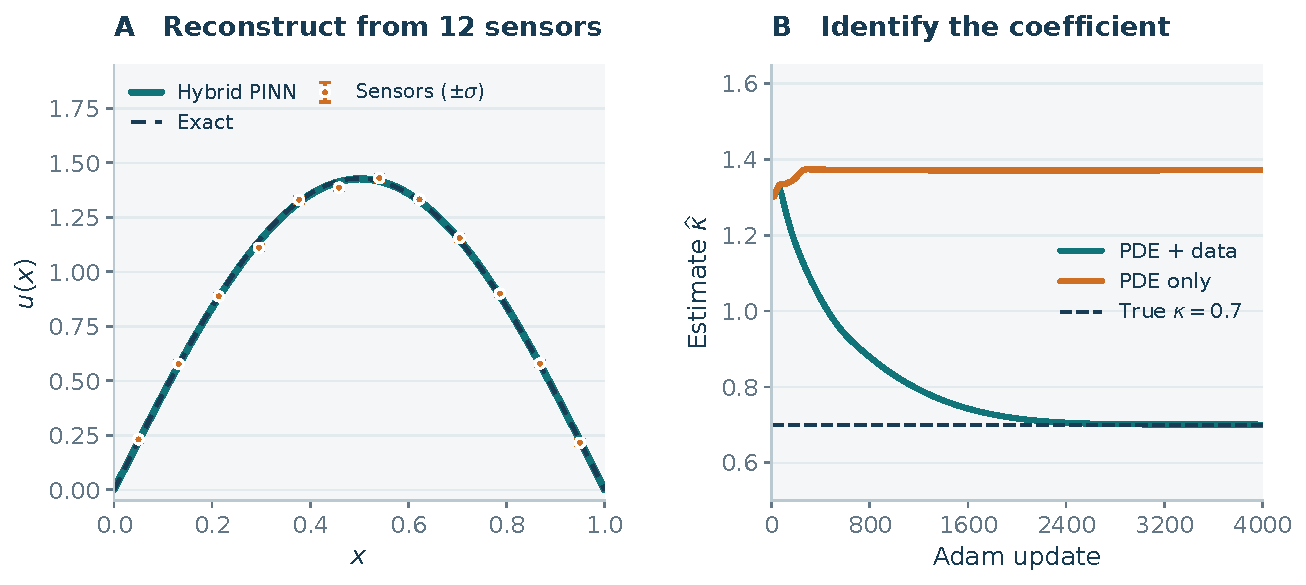
\includegraphics[width=\textwidth]{experiments/figures/inverse_recovery.pdf}
\begin{block}{Results for this noise realization}
Learned $\widehat\kappa=\textbf{\InverseKappa}$ (truth $0.7$);
coefficient error \textbf{\InverseKappaError}.
Relative field $L^2$ error: \textbf{\InverseLtwo}.
\end{block}
\labnote{The coefficient curve shows Adam iterations; the final values include
L-BFGS refinement. Noise level and optimizer settings are recorded with the results.}
\end{frame}

\renewcommand{\slideid}{L3-PY12}
\begin{frame}[c]{Python output: why the observations are essential}
\small
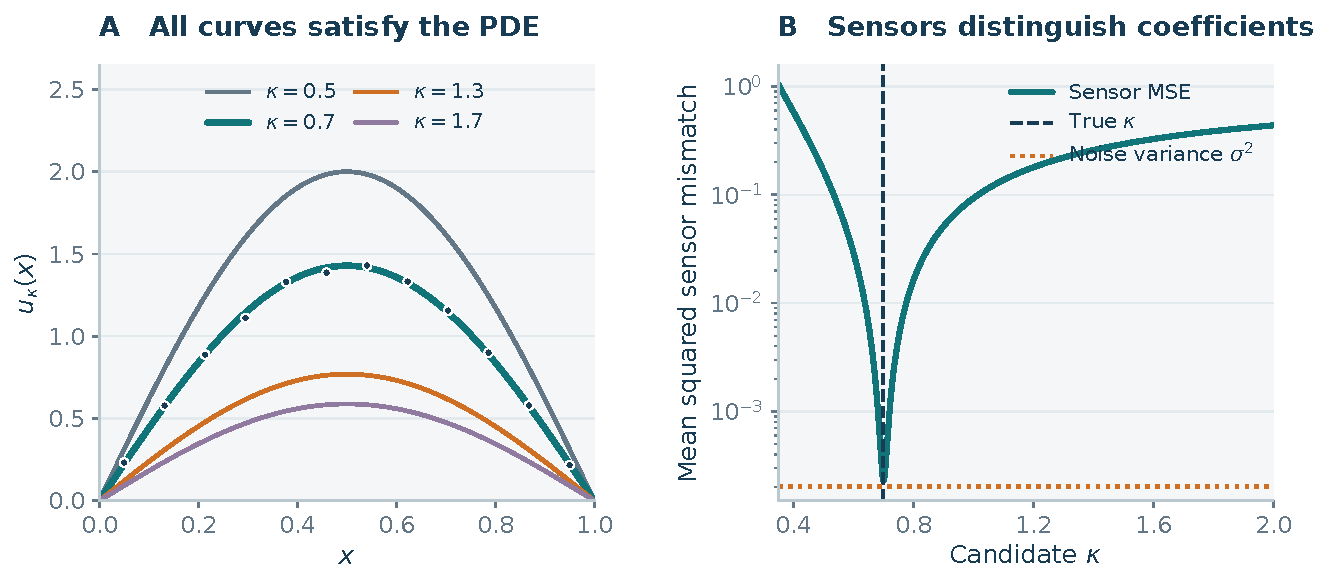
\includegraphics[width=\textwidth]{experiments/figures/inverse_identifiability.pdf}
\begin{block}{The PDE and boundary data leave a family of solutions}
For every $\kappa>0$, $u_\kappa(x)=\sin(\pi x)/\kappa$ solves the PDE.
Interior observations select a coefficient within this family.
\end{block}
\labnote{The right panel evaluates the analytic solution family at the noisy
sensors to show which coefficients fit the observations.}
\end{frame}
\renewcommand{\slideid}{L3}


% References and claim scope: experiments/limitations_sources.md.
\renewcommand{\slideid}{L3}
\section{Why classical solvers remain essential}

\renewcommand{\slideid}{L3-C01}
\begin{frame}[c]{Why classical numerical methods are still used}
\small
\guidingquestion{Can we reach a requested error tolerance at a predictable cost?}
\begin{slideitems}
\item \textbf{Controlled refinement:} mesh size, polynomial degree, and time step
give systematic ways to improve a discretization.
\item \textbf{Efficient algebra:} sparse matrices, preconditioners, and multigrid
exploit the structure of many PDEs.
\item \textbf{Physical structure:} appropriate finite-volume, mixed, or compatible
schemes can enforce conservation or other identities by construction.
\item \textbf{Established practice:} error estimation, complex geometry handling,
and extensively tested implementations.
\end{slideitems}
\begin{block}{A published benchmark}
In the PDE benchmarks of Grossmann et al., PINNs did not beat FEM in
solution time and accuracy on the problems tested.
\end{block}
\labnote{\href{https://arxiv.org/abs/2302.04107}{Grossmann et al., IMA J. Applied Mathematics (2024).}}
\end{frame}

\renewcommand{\slideid}{L3-C02}
\begin{frame}[c]{A classical route from approximation to accuracy}
\small
For conforming FEM ($V_h\subset V$) with bounded, coercive $a$,
C\'ea's lemma gives
\[
 \norm{u-u_h}_V\le \frac{M}{\alpha}
       \inf_{v_h\in V_h}\norm{u-v_h}_V.
\]
Here $M$ is the continuity constant and $\alpha>0$ the coercivity constant;
$u_h$ is the exactly solved Galerkin approximation.
\begin{slideitems}
\item With sufficient regularity and suitable meshes, approximation estimates
turn this into an explicit rate in $h$ and polynomial degree.
\item Reliable a posteriori estimators are available for many problem classes
and can guide local refinement.
\end{slideitems}
\begin{block}{A finite-tolerance solve still needs an error budget}
\[
\norm{u-\widetilde u_h}_V
\le \underbrace{\norm{u-u_h}_V}_{\text{discretization}}
  + \underbrace{\norm{u_h-\widetilde u_h}_V}_{\text{algebraic solve}}.
\]
Nonlinear, singular, or unstable problems still require appropriate analysis.
\end{block}
\end{frame}

\renewcommand{\slideid}{L3-C03}
\begin{frame}[c]{What a PINN error bound requires}
\small
\begin{block}{An error estimate under two assumptions}
If PDE stability gives $\norm{u-u_\theta}_X\le C_{\rm stab}\sqrt{\Loss(\theta)}$
and sampling gives $\Loss(\theta)\le\widehat\Loss(\theta)+\varepsilon_Q$, then
\[
 \norm{u-u_\theta}_X\le
 C_{\rm stab}\sqrt{\widehat\Loss(\theta)+\varepsilon_Q}.
\]
The loss must include the right residual and boundary norms for this PDE.
\end{block}
\begin{slideitems}
\item \textbf{Representation:} a good network may exist; training need not find it.
\item \textbf{Sampling:} a useful $\varepsilon_Q$ requires regularity and coverage,
with control valid for the network selected by training.
\item \textbf{Optimization:} a bound assuming small training error does not
prove Adam or L-BFGS reaches it at an affordable cost.
\end{slideitems}
\labnote{\href{https://arxiv.org/abs/2006.16144}{Mishra--Molinaro (2023)};
\href{https://doi.org/10.1017/S0962492923000089}{De Ryck--Mishra, Acta Numerica (2024)}.
Norms, rates, and constants depend on the PDE and formulation.}
\end{frame}

\renewcommand{\slideid}{L3-C05}
\begin{frame}[c]{Small training loss can still hide a wrong solution}
\small
\renewcommand{\arraystretch}{1.35}
\begin{tabular}{@{}>{\raggedright\arraybackslash}p{0.30\textwidth}>{\raggedright\arraybackslash}p{0.65\textwidth}@{}}
\toprule
Difficulty & What can go wrong\\
\midrule
Finite collocation & Residual peaks or thin layers fall between training points.\\
Multiple scales & Oscillations and sharp features can learn much more slowly
than the smooth background.\\
Time dependence & Small early-time errors and an unbalanced space--time loss
can spoil long-time predictions.\\
Physical constraints & A generic pointwise loss does not exactly impose cell
conservation, positivity, or an entropy inequality.\\
\bottomrule
\end{tabular}
\begin{block}{Adding data does not remove these issues}
Noisy or sparse observations introduce their own weighting and
identifiability questions, as the inverse experiment demonstrated.
\end{block}
\labnote{\href{https://arxiv.org/abs/2109.01050}{Krishnapriyan et al., NeurIPS (2021)};
\href{https://arxiv.org/abs/2007.14527}{Wang--Yu--Perdikaris, JCP (2022)}.
These are possible failure modes, not unavoidable outcomes.}
\end{frame}

\renewcommand{\slideid}{L3-C09}
\begin{frame}[c]{What helps PINNs, and what still needs checking}
\small
\renewcommand{\arraystretch}{1.4}
\begin{tabular}{@{}>{\raggedright\arraybackslash}p{0.41\textwidth}>{\raggedright\arraybackslash}p{0.54\textwidth}@{}}
\toprule
Possible improvement & Remaining check\\
\midrule
Hard boundary constraints & Interior PDE accuracy and ansatz suitability.\\
Adaptive collocation & Independent residual evaluation and correct sampling weights.\\
Feature scaling, domain splitting & Resolution of every relevant physical scale.\\
Better conditioning and optimizers & Actual solution error; convergence is still problem-dependent.\\
Weak or variational formulations & Stability, quadrature, and the chosen test space.\\
\bottomrule
\end{tabular}
\begin{block}{Check whether the change helps}
Measure the solution error before and after each change. Improvements
depend on the PDE, sampling, and training setup.
\end{block}
\labnote{\href{https://doi.org/10.1017/S0962492923000089}{De Ryck--Mishra (2024)};
\href{https://proceedings.mlr.press/v235/rathore24a.html}{Rathore et al. (2024)}.}
\end{frame}

\renewcommand{\slideid}{L3-C11}
\begin{frame}[c]{Where neural PDE solvers can have an advantage}
\small
\begin{slideitems}
\setlength\itemsep{0.8em}
\item \textbf{High-dimensional settings.} Neural representations and stochastic
sampling avoid the exponential size of tensor grids. For PDEs with exploitable
structure, this can make otherwise infeasible computations practical.
\item \textbf{Inverse problems with sparse or poorly distributed data.}
Jointly fit the state and unknown coefficients, using the PDE to constrain
regions with few measurements. This can avoid repeated full forward solves;
identifiability still requires informative observations.
\item \textbf{Complex geometry.} Meshfree formulations use interior and boundary
samples, reducing volume-meshing and remeshing effort for intricate or changing
domains. Accurate boundary representation and enforcement remain essential.
\end{slideitems}
\par\medskip
Compare total cost at matched accuracy, including training and geometry preparation.
\par\medskip
\labnote{Examples: \href{https://arxiv.org/abs/1707.02568}{Han--Jentzen--E (2018)};
\href{https://doi.org/10.1126/science.aaw4741}{Raissi et al. (2020)};
\href{https://arxiv.org/abs/2104.08426}{Sukumar--Srivastava (2022)}.}
\end{frame}

\renewcommand{\slideid}{L3}


\section{Checking a neural solution}
\subsection{Formulation and error checks}
\renewcommand{\slideid}{L3-S115}
\begin{frame}[c]{What to choose and what to check}
\small
\begin{slideitems}
\item Nondimensionalise the PDE and choose a strong, weak, or energy formulation.
\item Match the activation to the required derivatives; choose penalty or hard boundary enforcement.
\item Track each loss component and its parameter-gradient magnitude:
\end{slideitems}
\[
\widehat\Loss_j(\theta_k),\quad
\norm{\nabla_\theta\widehat\Loss_j(\theta_k)},\qquad j\in\{r,b,d\}.
\]
\begin{block}{Check the computed solution}
Check boundary, conservation, and other physical diagnostics on independent points.
If an exact solution is available, also monitor
\[
\norm{u_{\theta_k}-u}_{L^2},\qquad
\norm{u_{\theta_k}-u}_{H^1},\qquad
\norm{u_{\theta_k}-u}_{L^\infty}.
\]
\end{block}
\end{frame}

\renewcommand{\slideid}{L3-S117}
\begin{frame}[c]{Common failure modes}
\small
\guidingquestion{What should we ask when the loss decreases but the solution still looks wrong?}
\[
\begin{array}{rl}
\text{residual holes} & \Rightarrow \widehat\Loss_r\ll \Loss_r,\\[0.25em]
\text{boundary drift} & \Rightarrow \lambda_b\text{ too small},\\[0.25em]
\text{flat optimisation} & \Rightarrow \text{saturation/scaling},\\[0.25em]
\text{wrong branch} & \Rightarrow \text{nonuniqueness or poor initialisation}.
\end{array}
\]
\end{frame}

\renewcommand{\slideid}{L3-S118}
\begin{frame}[c]{Choosing among formulations}
\small
\guidingquestion{Which formulation matches the regularity, data, and PDE structure in front of us?}
\[
\begin{array}{lll}
\text{smooth solution + simple PDE} &\Rightarrow& \text{strong PINN},\\
\text{elliptic variational problem} &\Rightarrow& \text{Deep Ritz},\\
\text{low regularity or high order PDE} &\Rightarrow& \text{weak/variational PINN},\\
\text{sparse observations or inverse problem} &\Rightarrow& \text{hybrid data + PDE}.
\end{array}
\]
\end{frame}

\renewcommand{\slideid}{L3-S119}
\begin{frame}[c]{References}
\small
\begin{slideitems}
\item Raissi, Perdikaris, Karniadakis: physics-informed neural networks for forward and inverse PDE problems.
\item E and Yu: the Deep Ritz method for variational problems.
\item Kharazmi, Zhang, Karniadakis: variational PINNs and hp-VPINNs.
\end{slideitems}
\end{frame}

\end{document}
